\documentclass[9pt,letterpaper]{article}

\usepackage{caption}
\usepackage[utf8]{inputenc}
\usepackage[T1]{fontenc}
\usepackage[spanish]{babel}
\usepackage{geometry}
\usepackage{graphicx}
\usepackage{booktabs}
\usepackage{array}
\usepackage{tabularx}
\usepackage{float}
\usepackage{caption}
\usepackage{amsmath}
\usepackage{hyperref}

\geometry{margin=1.35cm}
\setlength{\parskip}{0.20em}
\setlength{\parindent}{0pt}
\captionsetup{font=footnotesize,labelfont=bf}
\renewcommand{\arraystretch}{1.05}

\title{\vspace{-1.3cm}\textbf{Determinantes ambientales de la diversidad de aves a escala microhábitat en Bogotá}}
\author{Miguel Ángel Camargo Mora}
\date{Estadística Multivariada y Modelos Lineales Aplicados}

\begin{document}
\maketitle
\vspace{-0.8cm}

\begin{abstract}
\small
Se evaluó la asociación entre la diversidad de aves urbanas y las condiciones ambientales horarias en Bogotá D.C., integrando listas completas de eBird con mediciones de la Red de Monitoreo de Calidad del Aire de Bogotá (RMCAB). La respuesta fue el índice de Shannon por evento de observación. Se construyó una base evento--ambiente mediante asignación espacio-temporal a la estación RMCAB más cercana ($\leq$5 km), se depuraron valores faltantes e imposibles, y se analizaron patrones mediante EDA, inferencia multivariable, regresión lineal múltiple y reducción de dimensión con PCA, PPCA y análisis factorial. Las listas de alta diversidad se asociaron con ambientes más húmedos, fríos y con menor ozono, viento y radiación solar, consistente con microhábitats vegetados y frescos. Dado que se rechazaron normalidad multivariada y homogeneidad de covarianzas, la comparación formal entre grupos se apoyó principalmente en una prueba permutacional de distancia entre centroides. La regresión confirmó que el esfuerzo de muestreo es el control central, pero que las variables ambientales mantienen señal significativa incluso después de incluirlo, lo que indica que el efecto del ambiente sobre la diversidad es real y no un artefacto de la ciencia ciudadana.
\end{abstract}

\section{Introducción}

La avifauna urbana es un indicador sensible del estado ecológico de las ciudades: responde a la heterogeneidad del hábitat, a gradientes de contaminación y a las condiciones meteorológicas con una resolución espacial y temporal difícil de obtener mediante otros grupos biológicos. Bogotá D.C., situada a 2\,600 m s.n.m. en la sabana cundiboyacense, representa un caso de estudio de particular interés: combina una altitud inusualmente elevada para una metrópoli latinoamericana, una marcada heterogeneidad de microhábitats (humedales tipo Ramsar, cerros orientales, parques urbanos, corredores de tráfico y zonas industriales) y una rica tradición de avistamiento de aves que alimenta plataformas de ciencia ciudadana como eBird con decenas de miles de listas al año.

Sin embargo, analizar esta diversidad requiere separar señales ecológicas genuinas de artefactos de muestreo. Las listas de eBird no son diseños experimentales controlados: el esfuerzo del observador ---duración de la salida, distancia recorrida, experiencia del birder--- co-varía con el número de especies reportadas de forma independiente a las condiciones ambientales. Al mismo tiempo, variables como la temperatura, la humedad, la radiación solar, el viento y los contaminantes del aire cambian simultáneamente a lo largo del día y entre zonas de la ciudad, creando estructuras de covarianza que solo son visibles con métodos multivariados.

El objetivo del estudio fue evaluar si las condiciones físico-químicas del ambiente urbano se asocian con la diversidad de aves reportada en eBird, una vez controlado el esfuerzo de muestreo. La pregunta estadística central fue: \textit{¿existen diferencias multivariadas entre el perfil ambiental de listas de baja y alta diversidad, y qué variables explican mejor la variabilidad del índice de Shannon después de controlar por esfuerzo de observación?}

\section{Datos y preparación}

\subsection{Fuentes y unidad de análisis}

La fuente ecológica fue eBird para Bogotá D.C. durante 2020--2025. Se conservaron únicamente listas completas con conteos numéricos, descartando registros con abundancias no cuantificadas. Para cada lista se calculó el índice de Shannon:
\[
H'=-\sum_i p_i\log(p_i),
\]
donde $p_i$ es la abundancia relativa de la especie $i$. También se conservaron riqueza de especies, duración de observación y distancia recorrida como variables de esfuerzo.

La fuente ambiental fue la RMCAB. Se procesaron cinco contaminantes: PM2.5, PM10, NO2, CO y O3; y cinco variables meteorológicas: temperatura, humedad, viento, radiación solar y precipitación. Cada lista de eBird se vinculó con la estación RMCAB más cercana dentro de un radio máximo de 5 km y con la medición correspondiente a la hora de inicio de la observación.

\begin{table}[H]
\centering
\caption{Diccionario de datos de las variables principales.}
\footnotesize
\begin{tabularx}{\linewidth}{p{3.0cm}p{2.4cm}X}
\toprule
Variable & Rol & Descripción \\
\midrule
\texttt{Shannon\_Index} & Respuesta & Índice de diversidad de Shannon calculado a partir de abundancias relativas por lista. \\
\texttt{Riqueza\_Especies} & Ecológica & Número de especies registradas en la lista. \\
\texttt{PM2.5}, \texttt{PM10} & Contaminantes & Material particulado fino y respirable medido por RMCAB. \\
\texttt{NO2}, \texttt{CO}, \texttt{O3} & Contaminantes & Gases asociados a combustión, calidad del aire y procesos fotoquímicos urbanos. \\
\texttt{Temperatura}, \texttt{Humedad} & Meteorológicas & Condiciones térmicas e higrométricas horarias. \\
\texttt{Viento}, \texttt{Radiacion\_Solar} & Meteorológicas & Intensidad del viento y radiación solar horaria. \\
\texttt{Lluvia} & Meteorológica & Indicador binario derivado de precipitación positiva. \\
\texttt{DURATION MINUTES} & Esfuerzo & Duración de la observación en minutos. \\
\texttt{EFFORT DISTANCE KM} & Esfuerzo & Distancia recorrida durante la lista. \\
\texttt{Distance\_to\_Station\_km} & Control espacial & Distancia entre la lista eBird y la estación RMCAB asignada. \\
\texttt{Diversidad\_Grupo} & Grupo & Clasificación por cuartiles de Shannon: baja, media o alta diversidad. \\
\bottomrule
\end{tabularx}
\end{table}

\subsection{Limpieza}

Los archivos RMCAB se encontraban en formato ancho, separados por variable, año y estación. Se transformaron a formato largo mediante \textit{melt}, indexado por fecha-hora y estación; se normalizaron nombres de estaciones y se consolidó una matriz ambiental horaria. Los valores no numéricos, etiquetas sin dato y valores físicamente imposibles se convirtieron a nulos; en CO se detectaron 7 valores negativos, tratados como mediciones inválidas.

El criterio para los análisis principales fue trabajar con casos completos según el método: 6\,178 observaciones para la matriz ambiental completa de 10 variables y 5\,298 para regresión con ambiente y esfuerzo completos. Los valores atípicos se marcaron mediante $|z|>3$, pero no se eliminaron automáticamente porque pueden representar episodios ambientales reales, como picos de contaminación o condiciones meteorológicas extremas. La precipitación se resumió como indicador \texttt{Lluvia} dado su fuerte concentración en cero.

\section{Métodos}

El análisis se organizó en cinco etapas. Primero, EDA para describir distribuciones, correlaciones y diferencias entre grupos extremos de Shannon. Segundo, distribuciones conjuntas y esperanzas condicionales para entender el comportamiento esperado de Shannon bajo combinaciones de temperatura y humedad. Tercero, comparación formal de centroides ambientales mediante pruebas multivariadas. Cuarto, regresión lineal múltiple con errores robustos HC3 para explicar Shannon controlando por esfuerzo. Quinto, PCA, PPCA y análisis factorial para resumir la estructura latente del ambiente urbano.

Para la inferencia multivariable se usaron nueve variables continuas estandarizadas: PM2.5, PM10, NO2, CO, O3, temperatura, humedad, viento y radiación solar. La variable lluvia se excluyó de esta comparación por ser binaria.

\section{Resultados}

\subsection{Análisis exploratorio}

El EDA mostró asimetría positiva en contaminantes como PM2.5, PM10, CO y O3, patrón típico de distribuciones con cola derecha por episodios puntuales de contaminación urbana. El índice de Shannon presentó una distribución unimodal levemente asimétrica a la izquierda (Q1$=1.71$, Q3$=2.60$), con un pico de masa cerca de $H'=2.2$--$2.4$ y una cola hacia valores bajos debida a listas de una o pocas especies. La concentración en cero de O3 (más de 2\,000 registros en el primer bin) y la bimodalidad de humedad (valle entre 40--70\% y pico en $\sim$85\%) son rasgos diagnósticos del clima de sabana de altura de Bogotá: la humedad es alta en la mañana, desciende al mediodía y sube nuevamente con las lluvias vespertinas, mientras el O3 solo se forma en las horas de máxima radiación UV. Lluvia fue esencialmente binaria (5\,839 eventos sin lluvia vs. 339 con lluvia), justificando su tratamiento como indicador dicotómico.

\begin{figure}[H]
    \centering
    \begin{minipage}{0.35\textwidth}
        \centering
        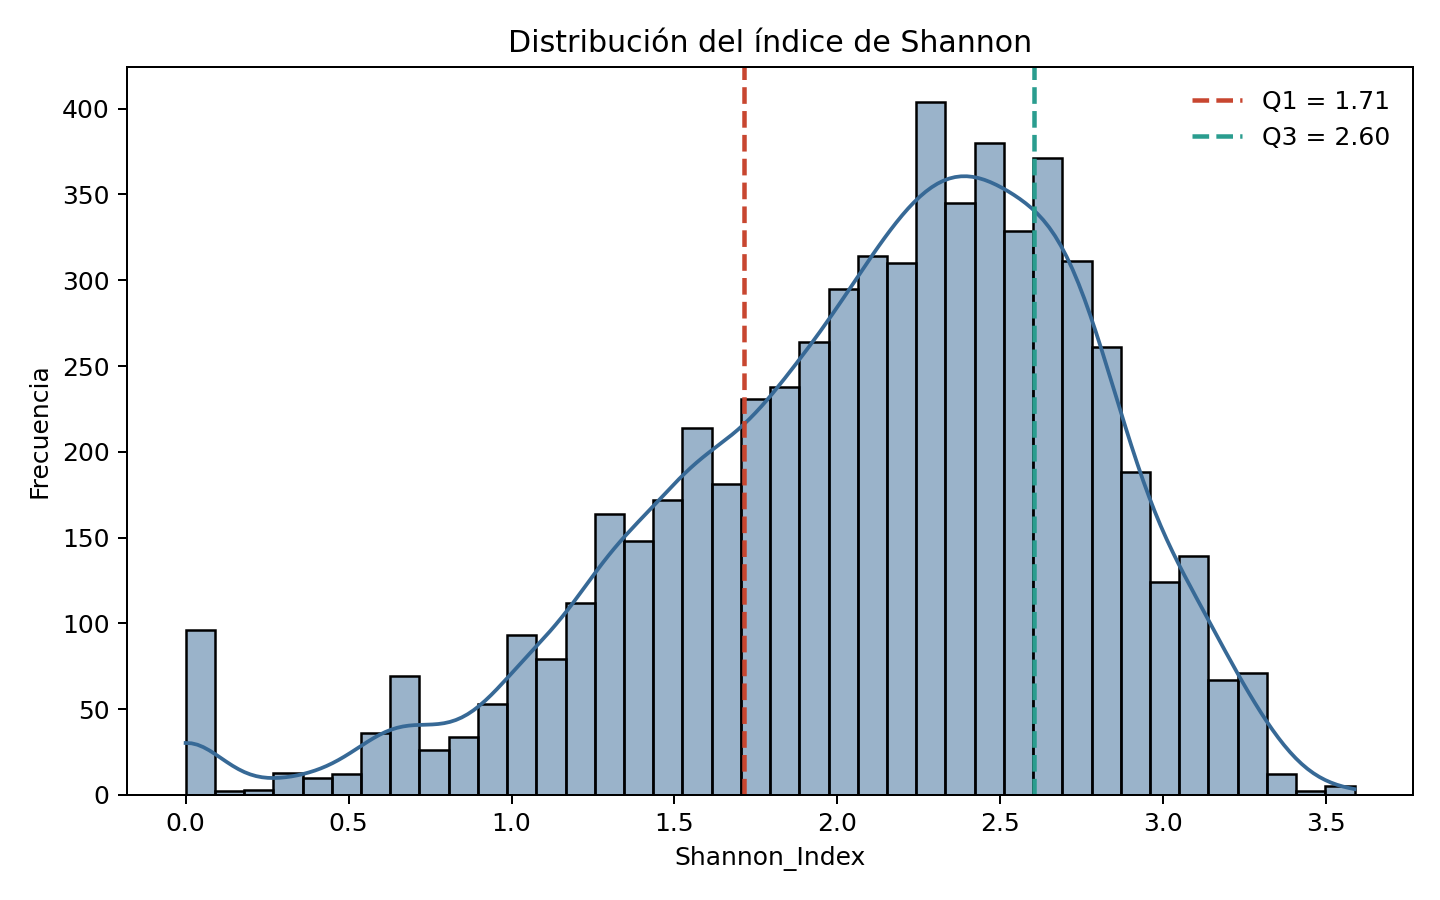
\includegraphics[width=\textwidth]{imagenes/01_shannon_distribution.png}
        \caption{Distribución del índice de Shannon con cuartiles Q1 y Q3.}
    \end{minipage}\hfill
    \begin{minipage}{0.62\textwidth}
        \centering
        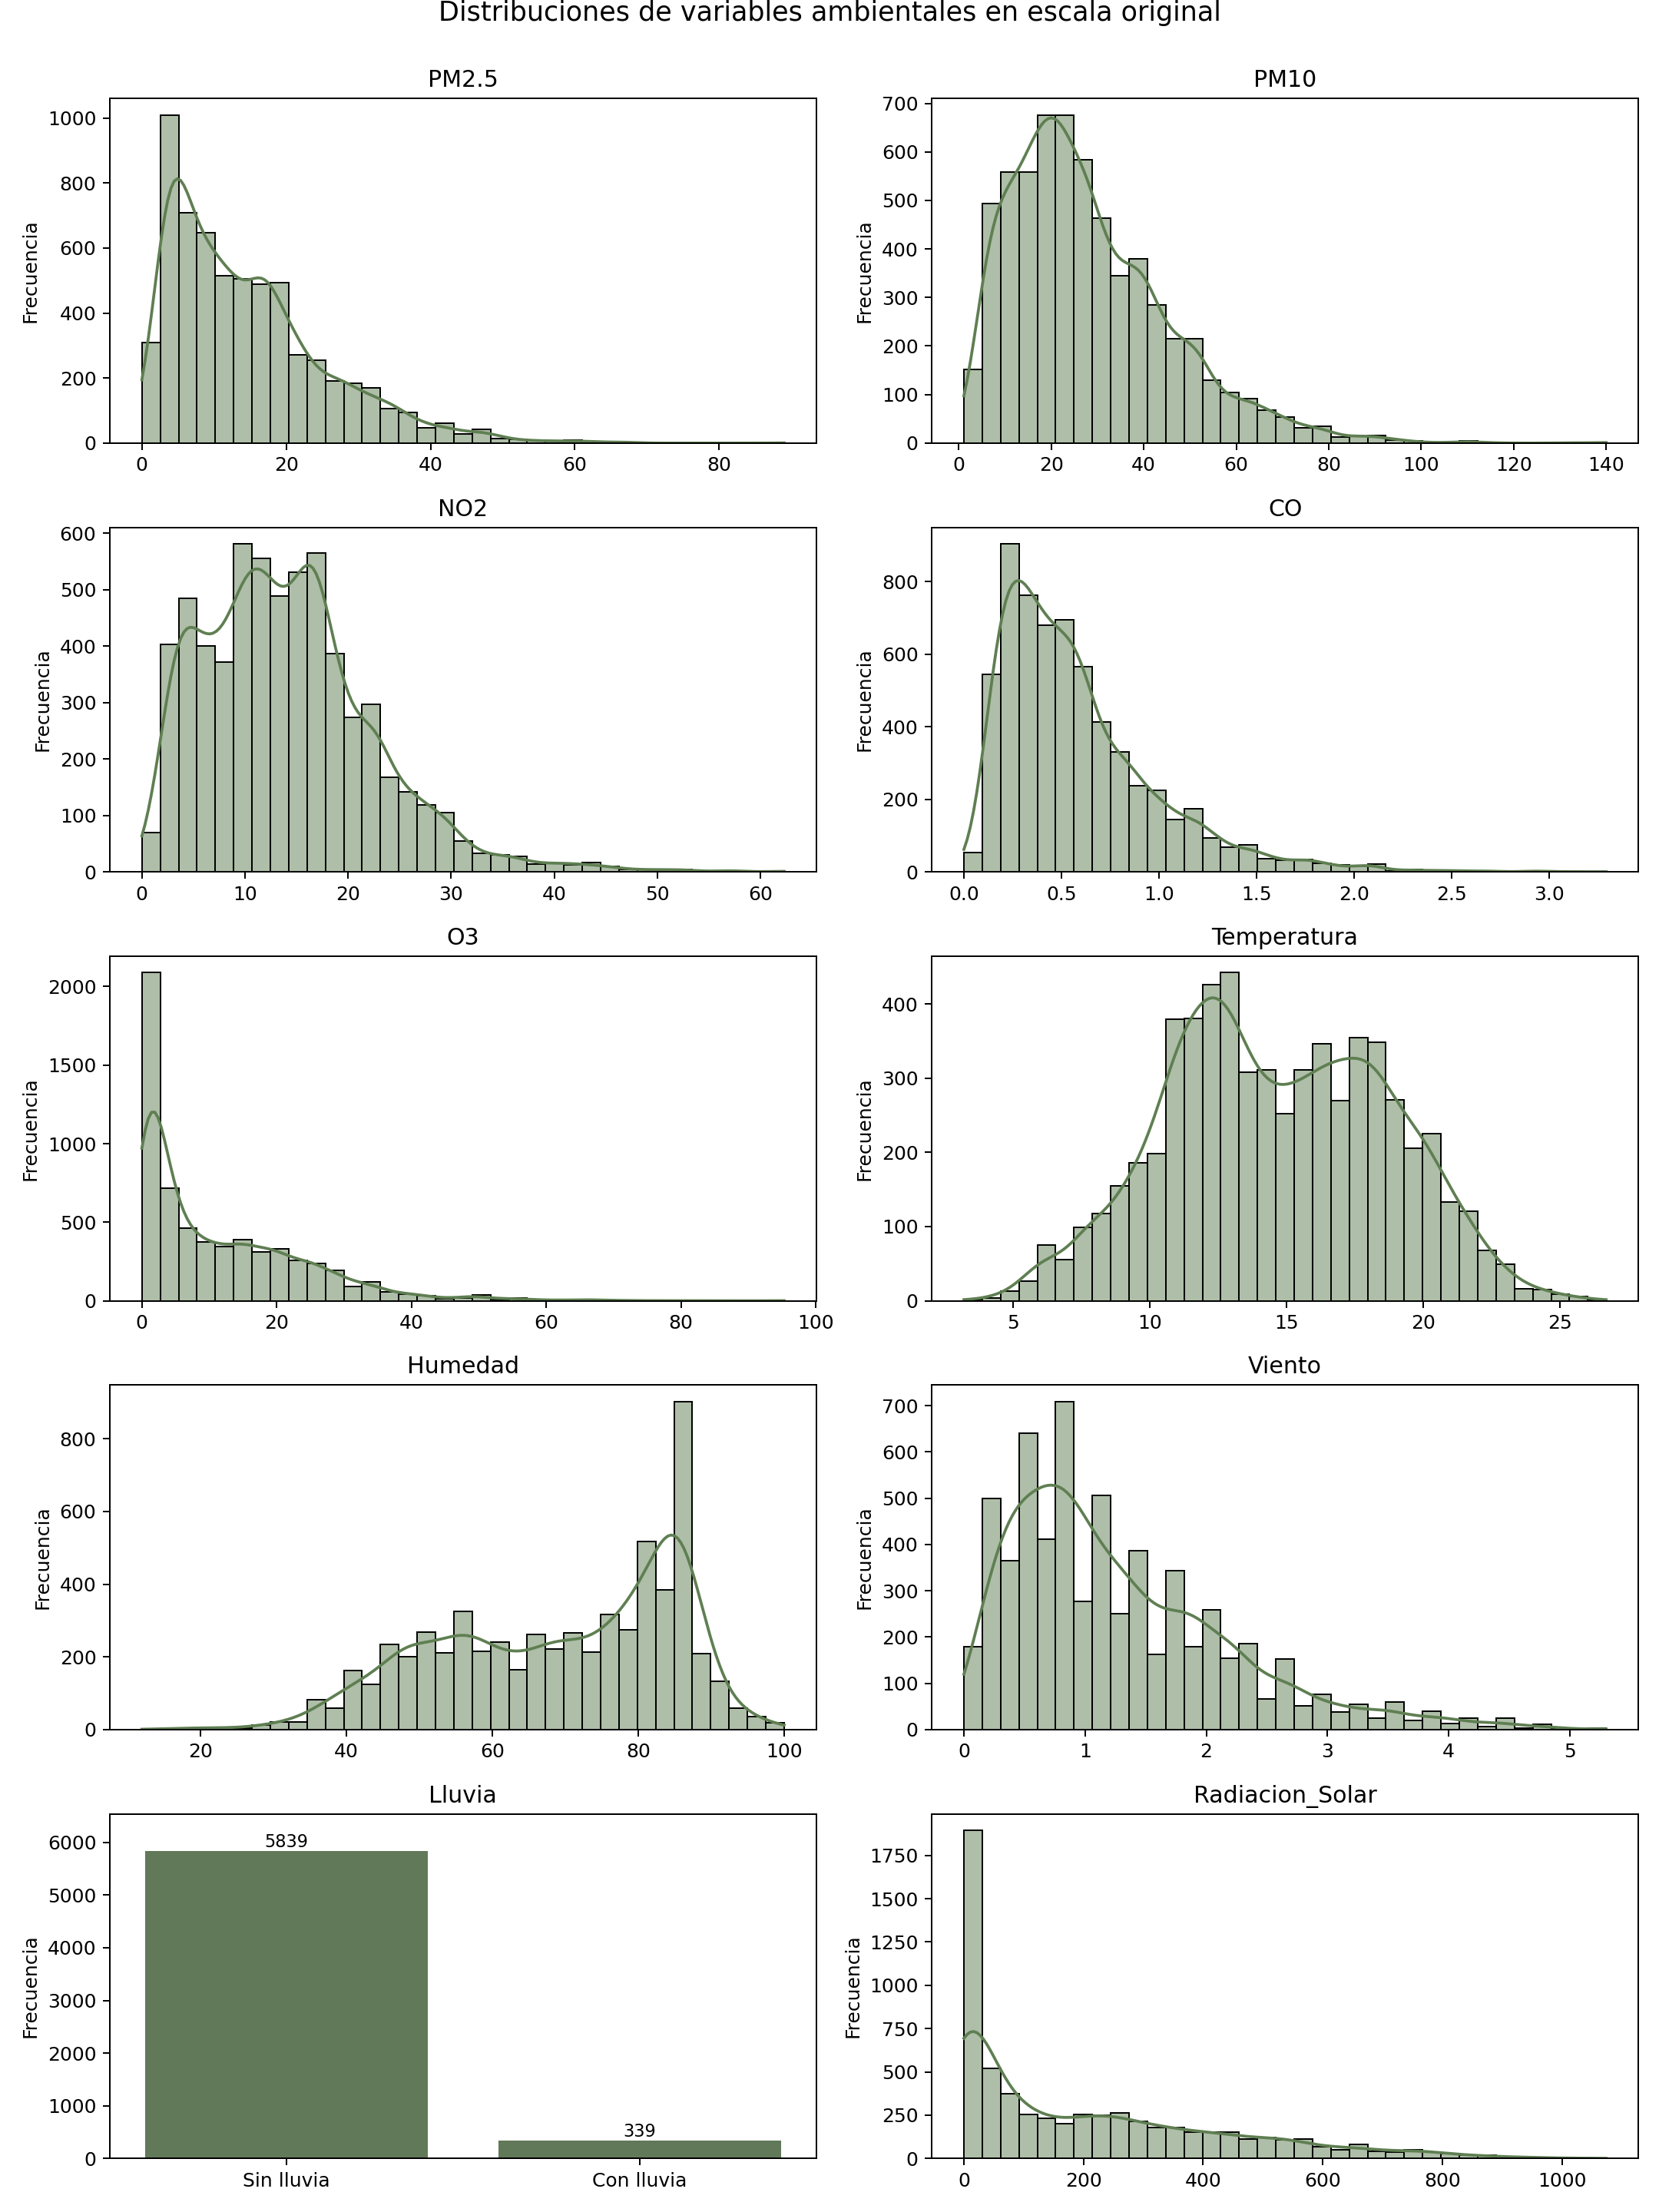
\includegraphics[width=\textwidth]{imagenes/02_environment_distributions_original.png}
        \caption{Distribuciones de las variables ambientales en escala original. Contaminantes y radiación muestran cola derecha; humedad presenta bimodalidad diurna; O3 concentra masa en cero.}
    \end{minipage}
\end{figure}

Las correlaciones de Pearson más altas con Shannon fueron riqueza de especies ($r=0.846$), temperatura ($r=-0.350$), humedad ($r=0.318$), O3 ($r=-0.297$), viento ($r=-0.276$) y radiación solar ($r=-0.273$). PM2.5 y PM10 tuvieron asociación marginal débil en el análisis bivariado, aunque su comportamiento cambia al controlar por otras variables en el modelo múltiple.

La comparación descriptiva entre grupos extremos reveló perfiles ambientales cualitativamente distintos: las listas de alta diversidad se registraron bajo menor temperatura media (12.89 vs.~16.80 °C), mayor humedad relativa (75.47 vs.~61.23\%), menor O3 (7.22 vs.~17.28 ppb), menor viento (0.98 vs.~1.68 m/s) y notablemente menor radiación solar (125.04 vs.~289.87 W/m²). Estas diferencias apuntan a condiciones propias de horas tempranas del día y de microhábitats con mayor cobertura vegetal.

\begin{figure}[H]
    \centering
    \begin{minipage}{0.48\textwidth}
        \centering
        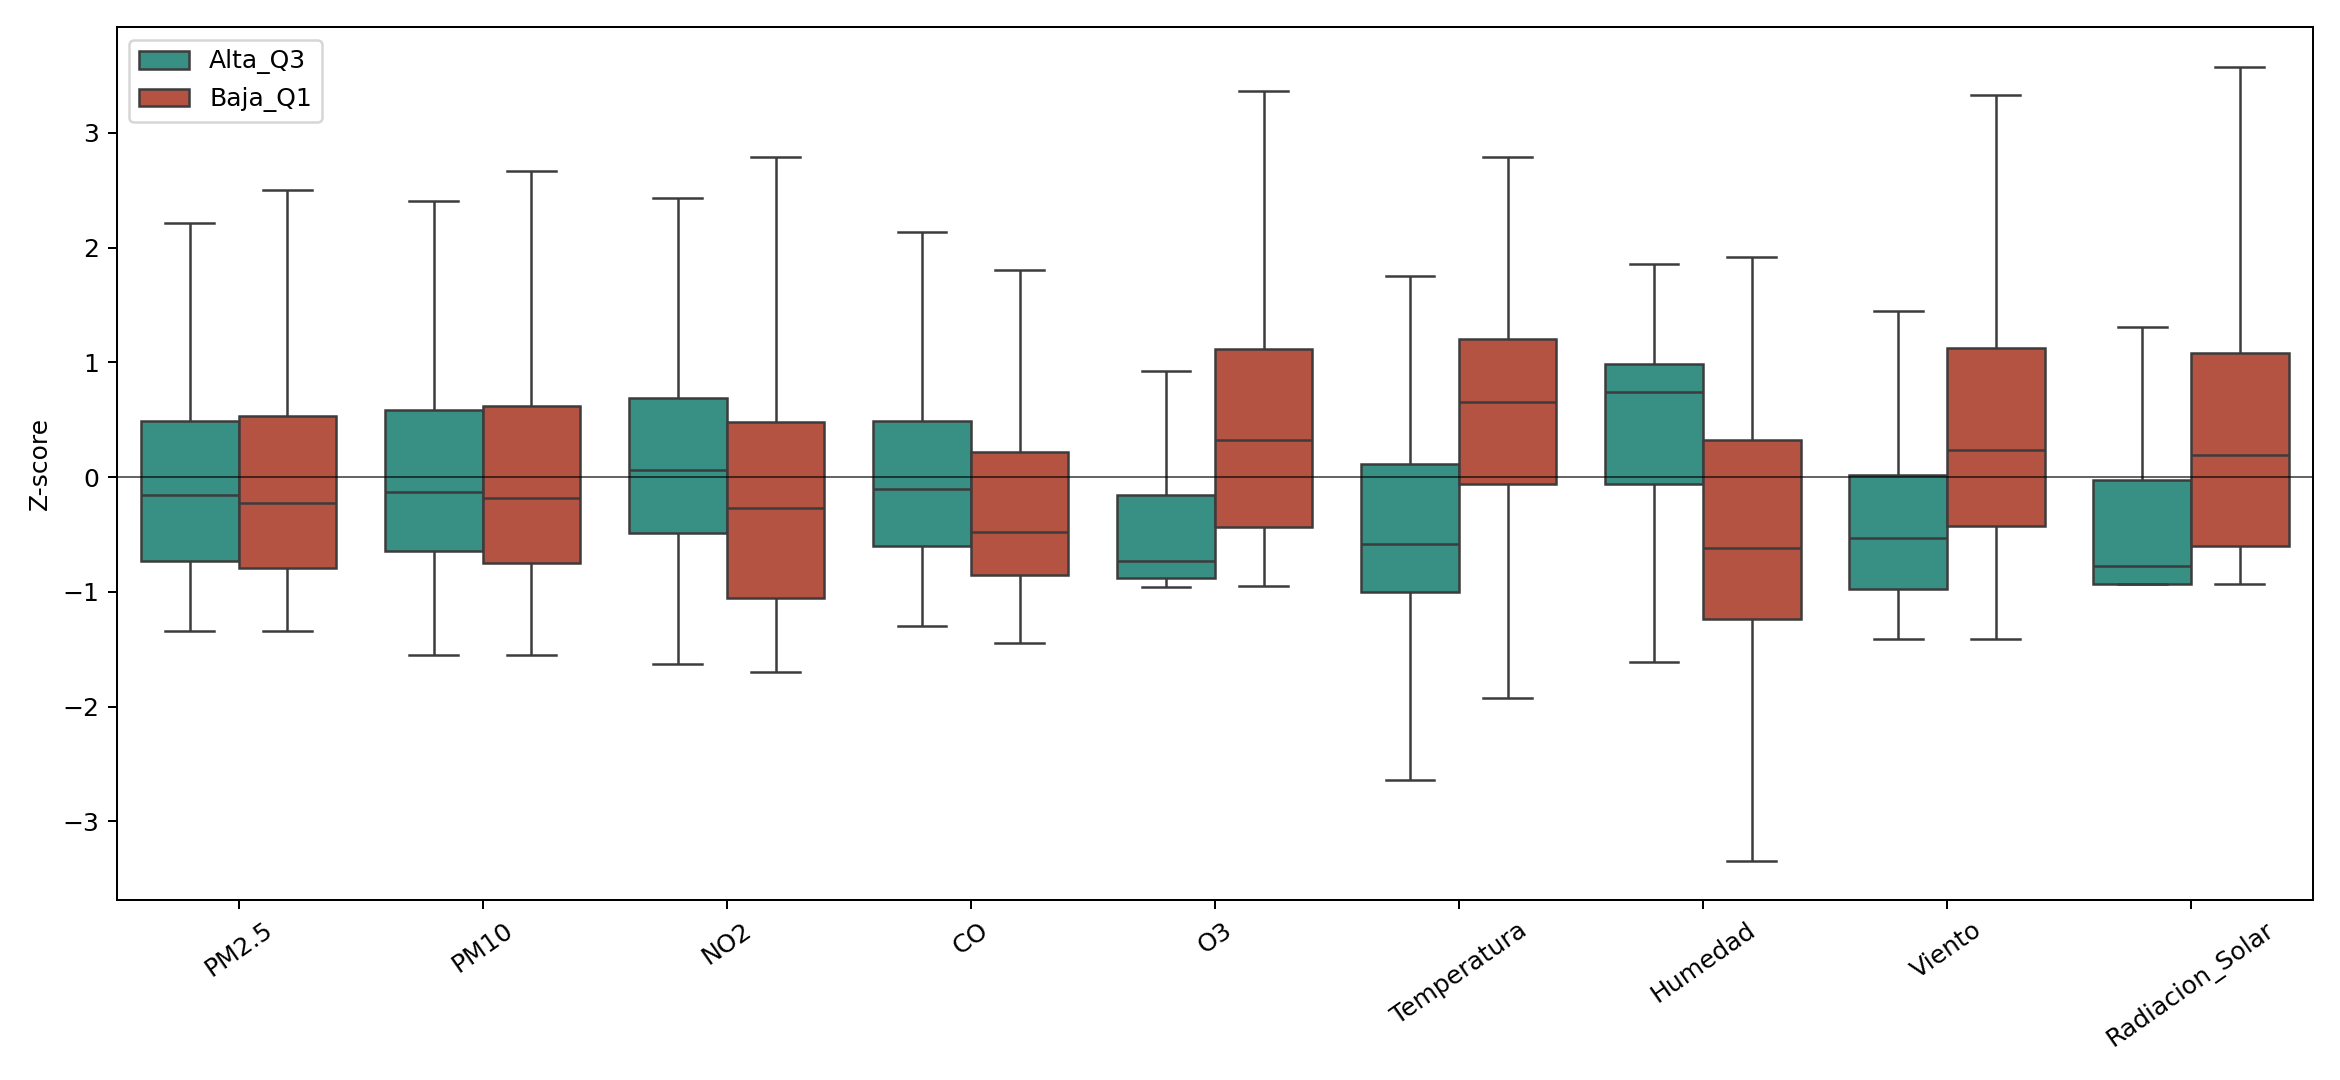
\includegraphics[width=\textwidth]{imagenes/eda_q1_q3_boxplots_z.png}
        \caption{Perfil ambiental estandarizado para baja y alta diversidad.}
    \end{minipage}\hfill
    \begin{minipage}{0.48\textwidth}
        \centering
        
\includegraphics[width=\textwidth]{Informe/imagenes/03_pearson_correlation_heatmap.png}
        \caption{Mapa de correlaciones entre variables ambientales y Shannon.}
    \end{minipage}
\end{figure}

\subsection{Distribuciones conjuntas y esperanza condicional}

La distribución conjunta de temperatura, humedad y Shannon, bajo una aproximación normal trivariada para el vector $(T,H,H')$, permitió derivar la superficie de esperanza condicional:
\[
E[H'|T,H]=2.112-0.0472(T-14.648)+0.0031(H-69.006).
\]

La matriz de covarianzas estimada mostró una relación negativa fuerte entre temperatura y humedad ($\operatorname{cov}=-55.221$), junto con covarianzas de Shannon negativas con temperatura ($-0.935$) y positivas con humedad ($3.407$). Esta estructura de covarianza es coherente con la dinámica diurna bogotana: la temperatura asciende desde el amanecer hacia el mediodía, mientras la humedad relativa desciende simultáneamente; los observadores que salen temprano, cuando el ambiente es más frío y húmedo, registran mayor diversidad. La correlación entre Shannon observado y su esperanza condicional fue 0.353 ($R^2\approx0.124$), lo que indica que el componente climático explica cerca de un 12\% de la variabilidad de Shannon de forma exclusiva, sin considerar el esfuerzo ni los contaminantes.

\begin{figure}[H]
\centering
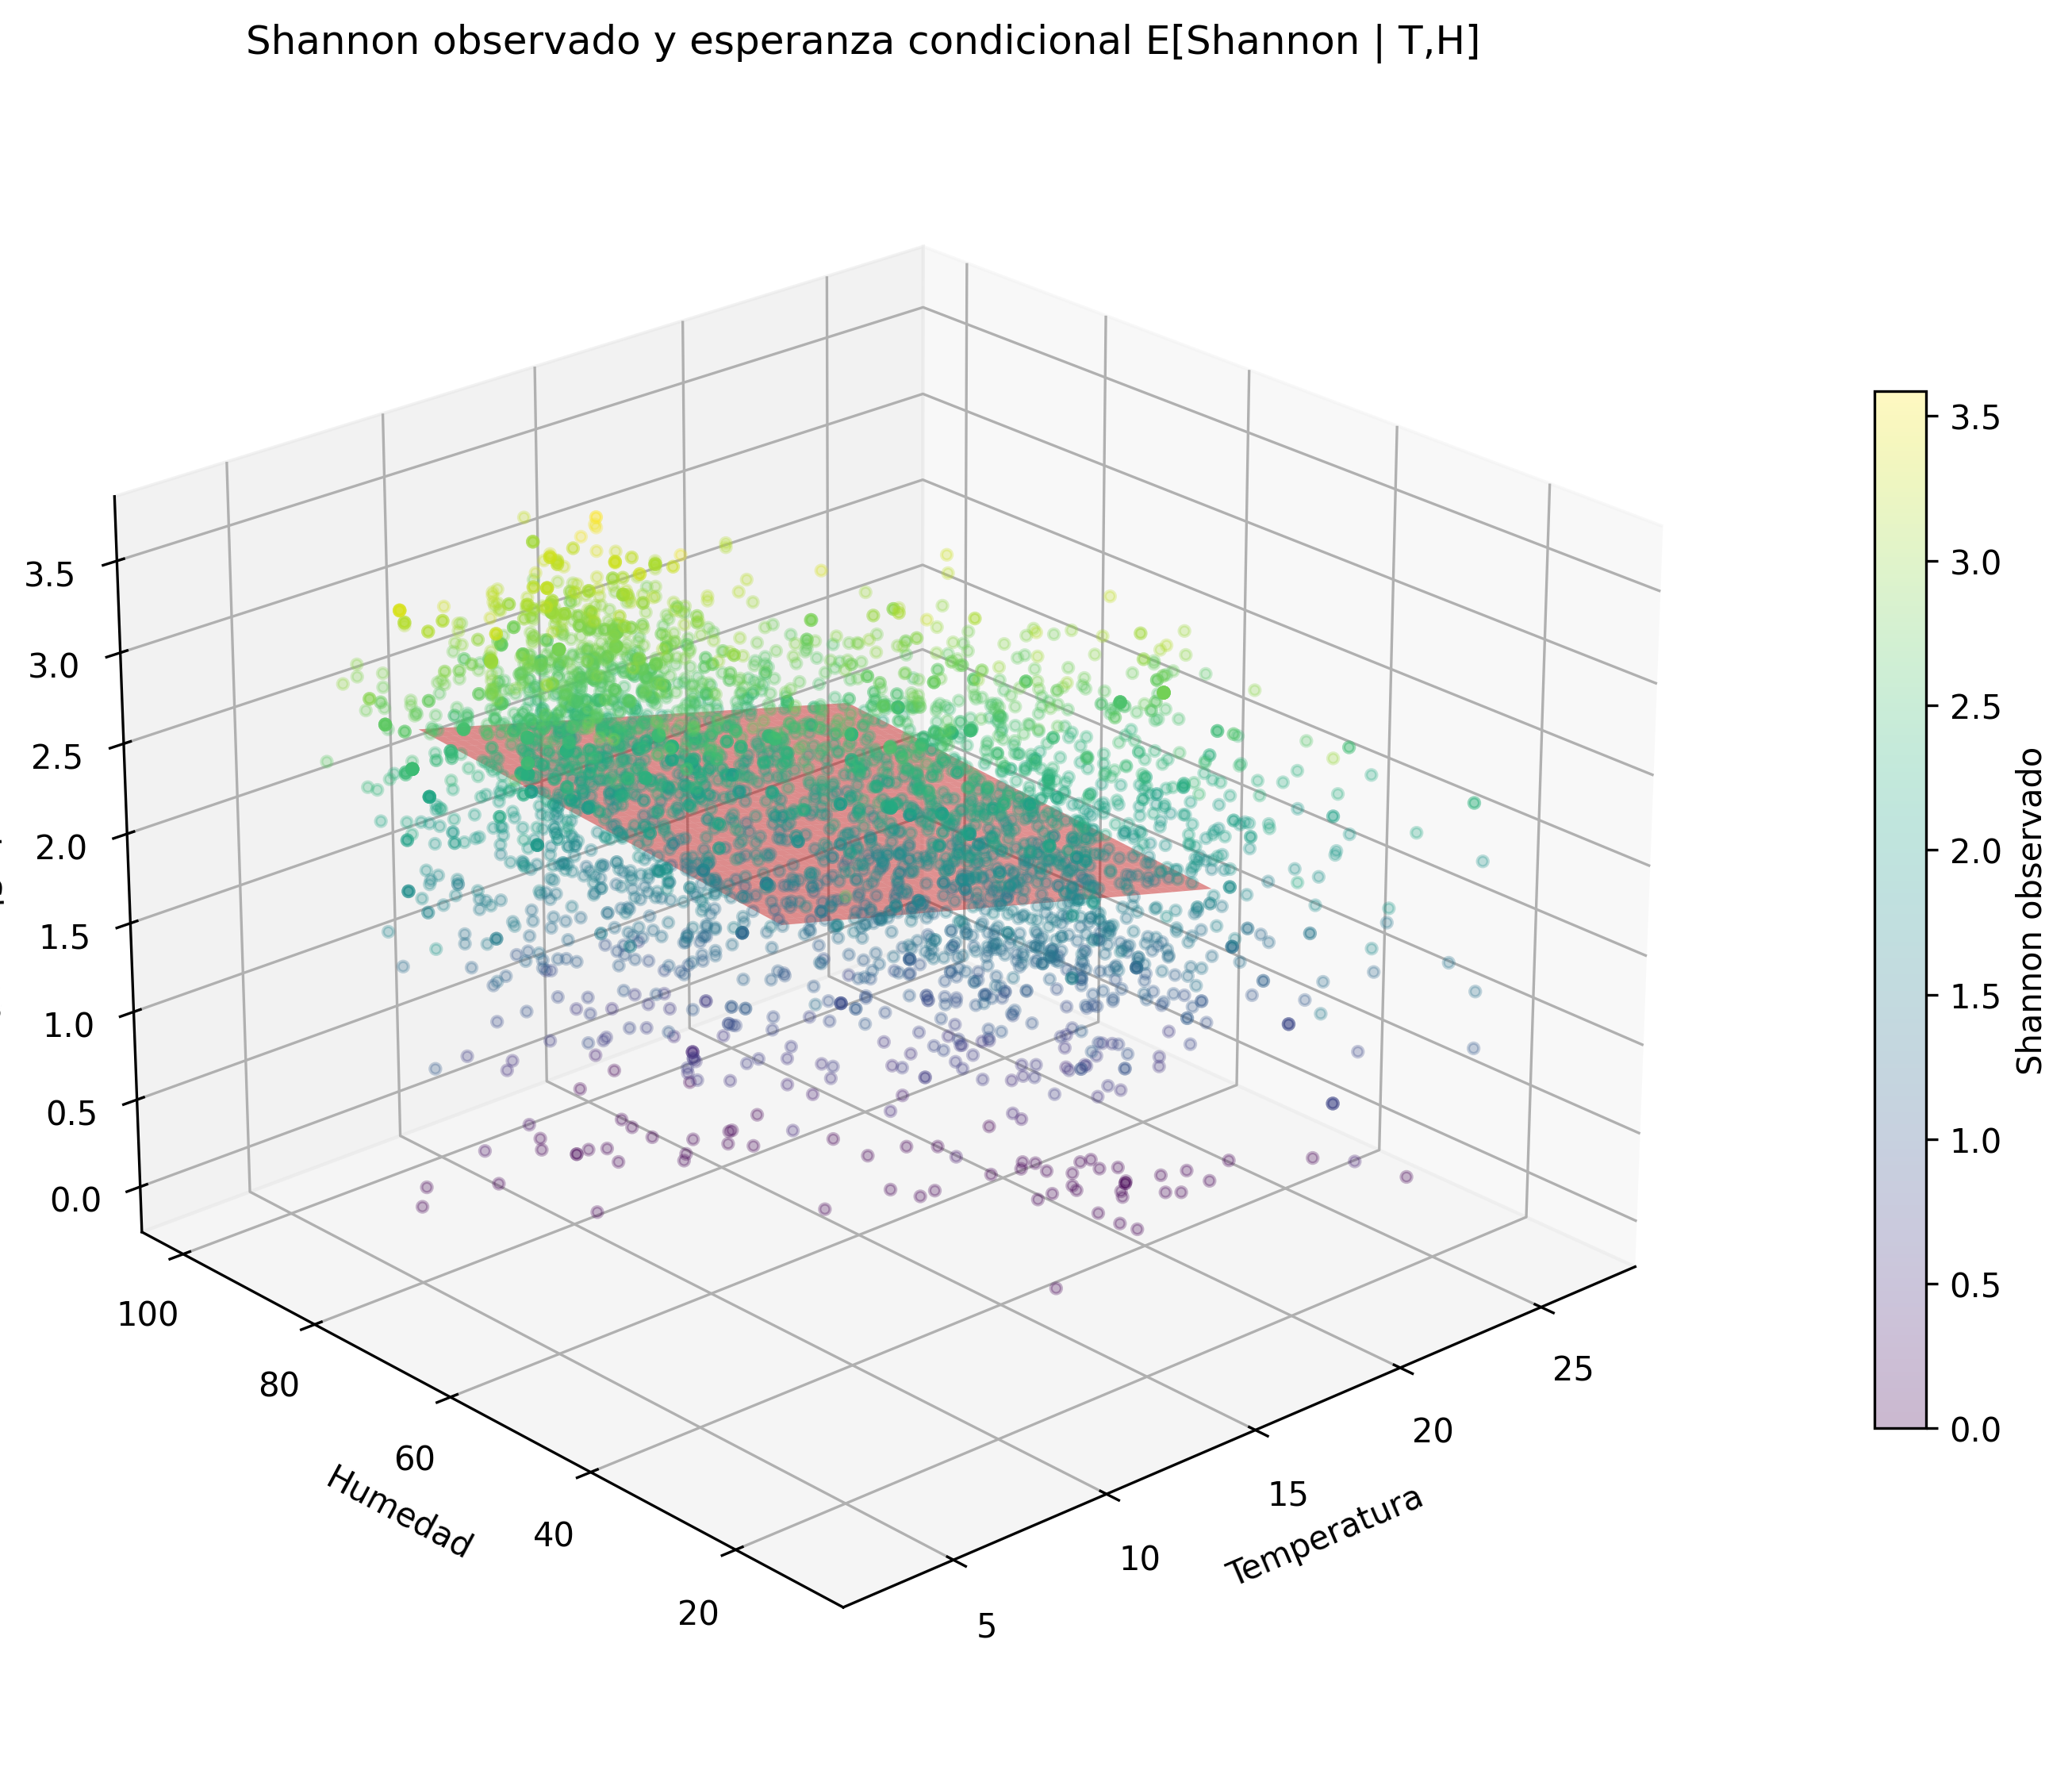
\includegraphics[width=0.52\linewidth]{imagenes/shannon_condicional_3d_temp_humedad.png}
\caption{Shannon observado y superficie de esperanza condicional $E[H'|T,H]$ bajo la normal trivariada temperatura--humedad--Shannon.}
\end{figure}

\subsection{Inferencia multivariable}

La comparación formal se planteó sobre los extremos de diversidad: baja diversidad ($n=1{,}075$, cuartil inferior) y alta diversidad ($n=1{,}760$, cuartil superior). Las hipótesis fueron:
\[
H_0:\boldsymbol{\mu}_{\text{baja}}=\boldsymbol{\mu}_{\text{alta}}, \quad H_A:\boldsymbol{\mu}_{\text{baja}}\neq\boldsymbol{\mu}_{\text{alta}},
\]
donde $\boldsymbol{\mu}$ representa el vector medio de las nueve variables ambientales continuas estandarizadas.

Mardia rechazó normalidad multivariada en ambos grupos ($p<0.001$). Box's M rechazó igualdad de matrices de covarianza ($\chi^2=1466.055$, gl=45, $p<0.001$). Hotelling $T^2$ detectó diferencia de centroides ($T^2=885.450$, $F=98.105$, $p<0.001$), pero se interpreta solo como referencia clásica dado el incumplimiento de sus supuestos.

La evidencia principal fue la prueba permutacional de distancia entre centroides (5\,000 simulaciones): la distancia observada fue 1.921 y el valor-$p$ permutacional fue $<0.001$, rechazando $H_0$. En términos sustantivos, los ambientes asociados a alta y baja diversidad están separados en el espacio multivariado de forma estadísticamente irrepetible por azar.

\begin{table}[H]
\centering
\caption{Diferencias medias estandarizadas entre alta y baja diversidad.}
\footnotesize
\begin{tabular}{lrrr}
\toprule
Variable & Alta & Baja \\
\midrule
Temperatura & -0.437 & 0.535 \\
O3 & -0.354 & 0.484 \\
Viento & -0.336 & 0.434 \\
Radiación solar & -0.363 & 0.388 \\
NO2 & 0.132 & -0.103 \\
Humedad & 0.400 & -0.481\\
\bottomrule
\end{tabular}
\end{table}

\begin{figure}[H]
\centering
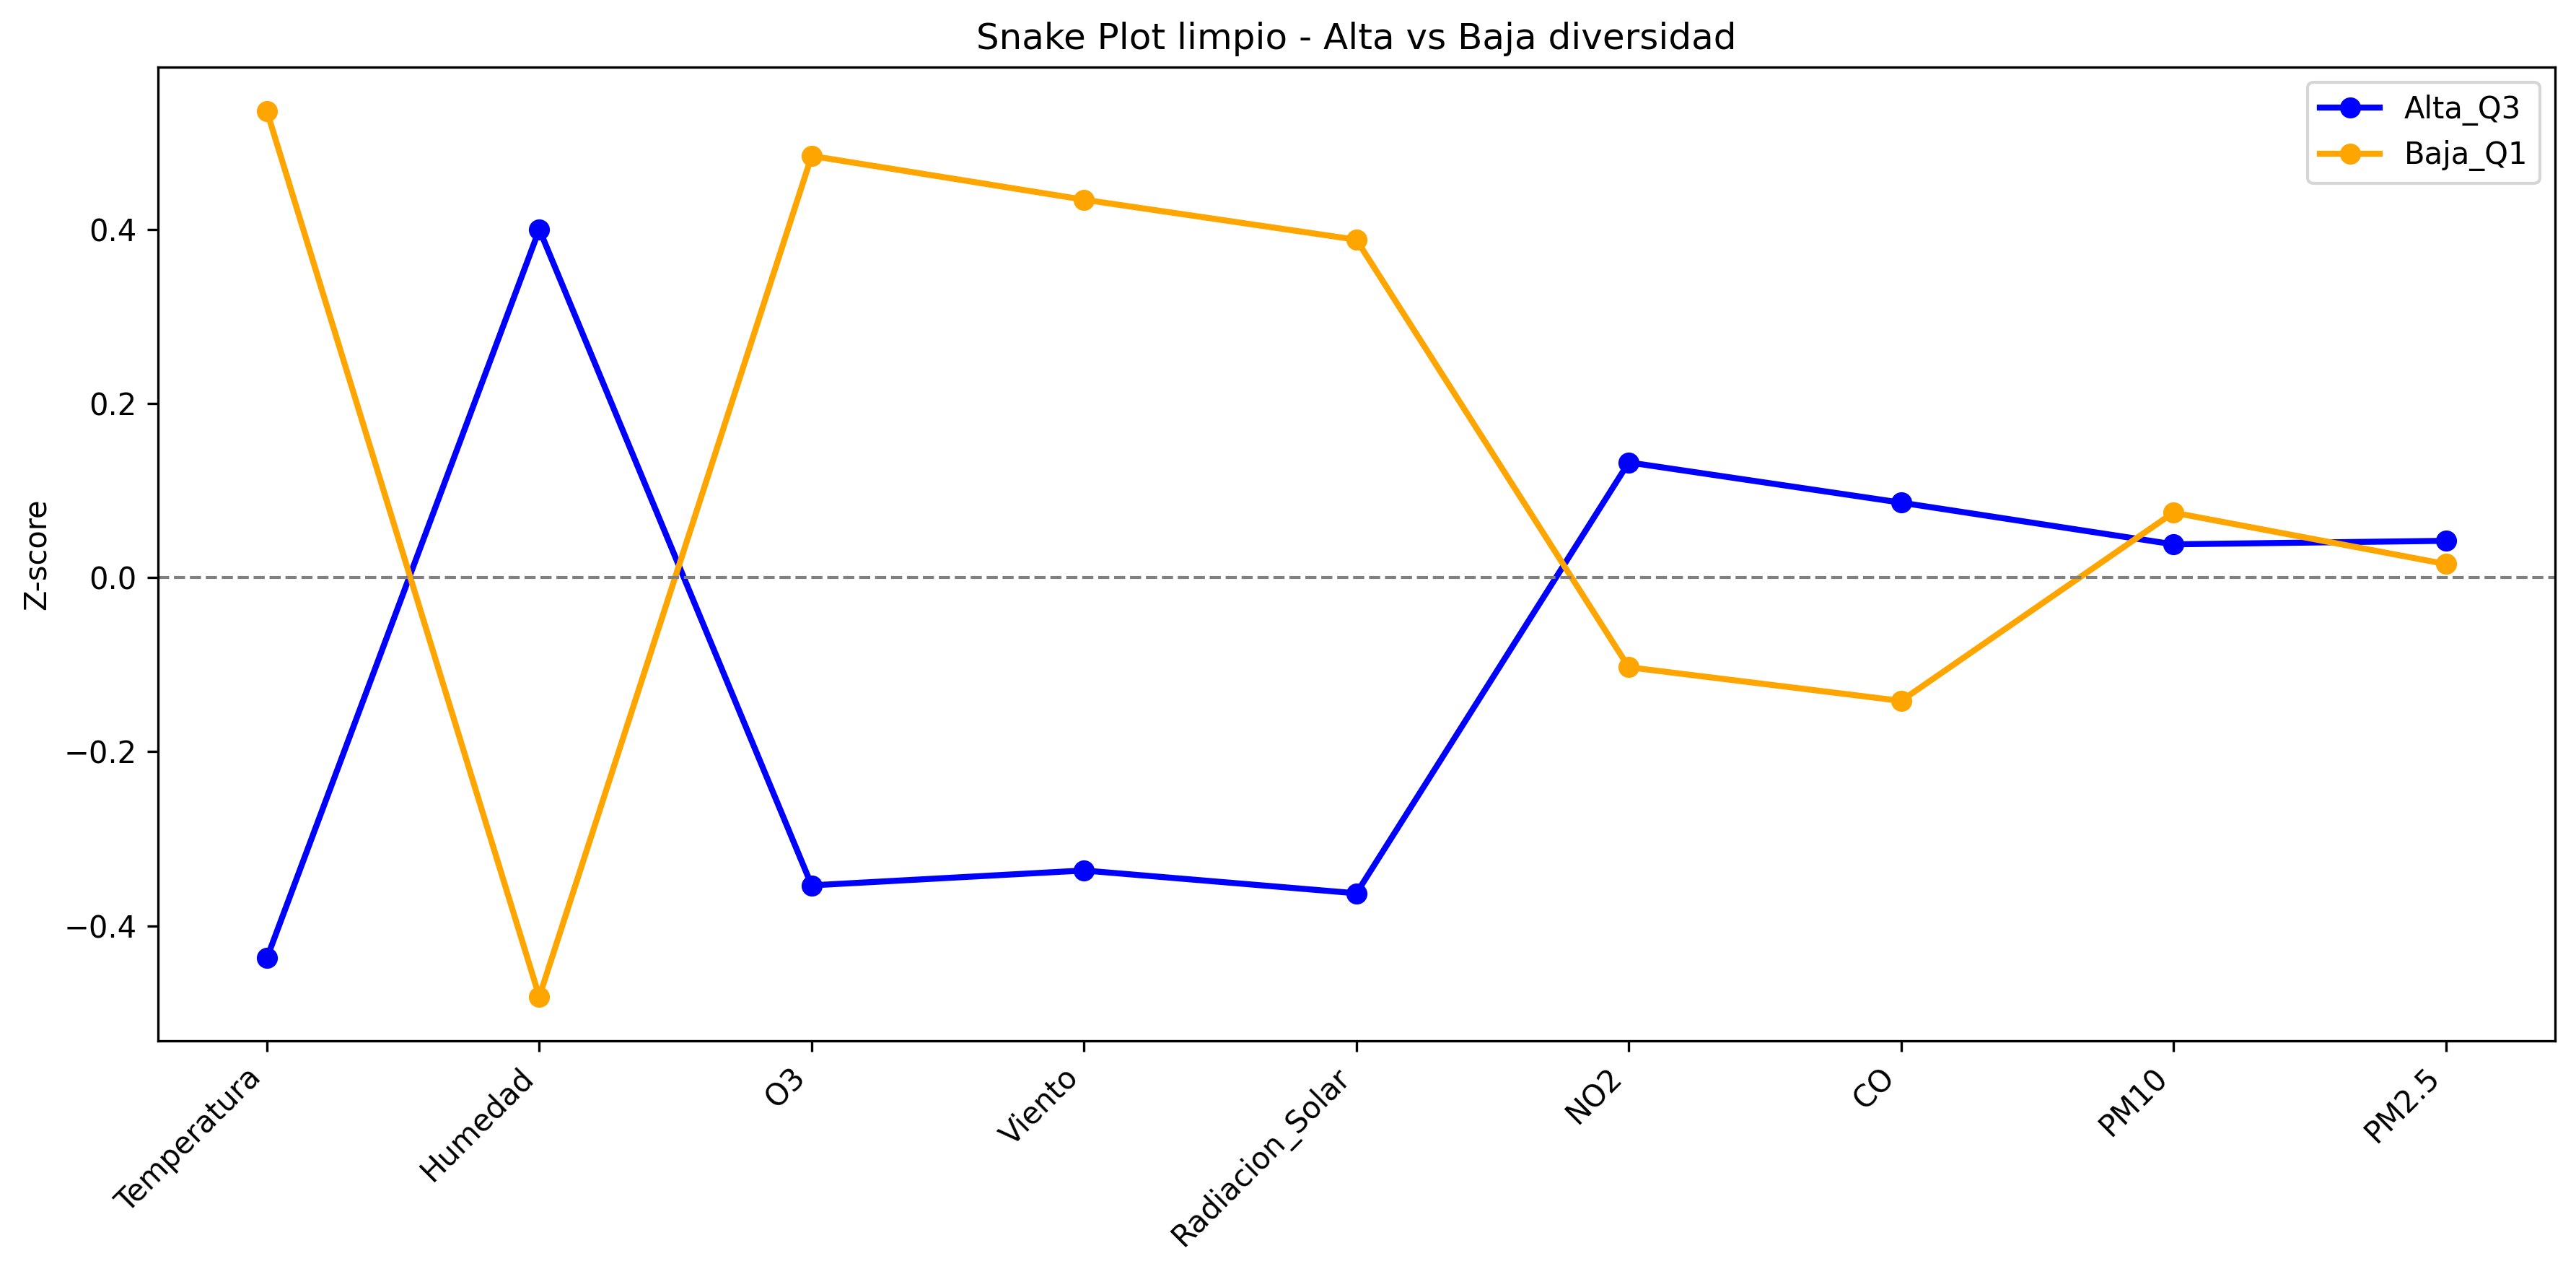
\includegraphics[width=0.48\linewidth]{imagenes/snake_plot_final.png}
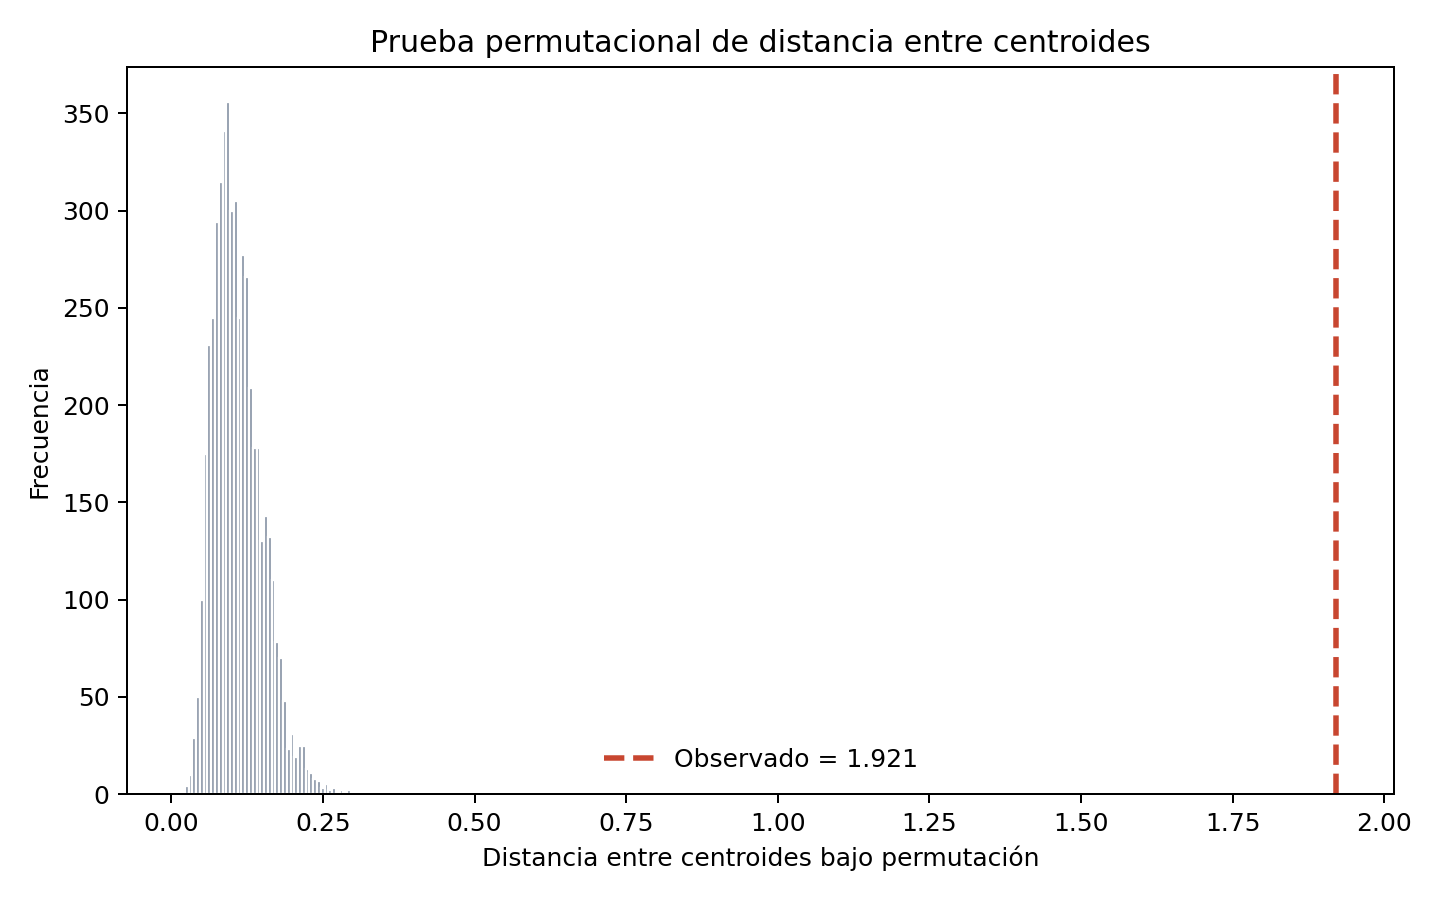
\includegraphics[width=0.48\linewidth]{imagenes/permutation_centroid_distance.png}
\caption{Izquierda: perfil multivariado medio por grupo. Derecha: distribución permutacional de la distancia entre centroides.}
\end{figure}

\subsection{Regresión lineal múltiple}

Se ajustó un modelo lineal con Shannon como respuesta:
\[
H' \sim \text{contaminantes}_z+\text{meteorología}_z+\text{duración}_z+\text{distancia}_z.
\]
El modelo se estimó con 5\,298 observaciones. El ajuste global fue significativo ($F=179.397$, $p<0.001$), con $R^2=0.289$ y $R^2$ ajustado $=0.288$.

\begin{table}[H]
\centering
\caption{Coeficientes estandarizados principales con inferencia robusta HC3.}
\footnotesize
\begin{tabular}{lrr}
\toprule
Variable & Coef. & Valor-p HC3 \\
\midrule
Duración & 0.225 & $<0.001$ \\
Humedad & 0.089 & $<0.001$ \\
Temperatura & -0.080 & $<0.001$ \\
Distancia & -0.057 & $<0.001$ \\
Viento & -0.050 & $<0.001$ \\
PM2.5 & 0.041 & 0.001 \\
O3 & -0.032 & 0.022 \\
CO & -0.029 & 0.005 \\
Lluvia & -0.025 & $<0.001$ \\
NO2 & -0.023 & 0.026 \\
PM10 & -0.021 & 0.116 \\
\bottomrule
\end{tabular}
\end{table}

Los diagnósticos rechazaron homocedasticidad (Breusch--Pagan $p<0.001$) y normalidad de residuos (Shapiro--Wilk $p<0.001$); Durbin--Watson fue 1.213, compatible con autocorrelación positiva leve. Por ello, la significancia se reportó con errores robustos HC3. La humedad tuvo el mayor VIF=5.321 y la temperatura VIF=4.780, reflejando colinealidad meteorológica moderada pero no preocupante. El análisis de sensibilidad sin humedad ($R^2$ ajustado=0.284) mostró que temperatura se hizo más negativa ($-0.121$) y O3 más negativo ($-0.057$), confirmando que humedad absorbe parte de la señal climática pero no la elimina.

\begin{figure}[H]
    \centering
    \begin{minipage}{0.48\textwidth}
        \centering
        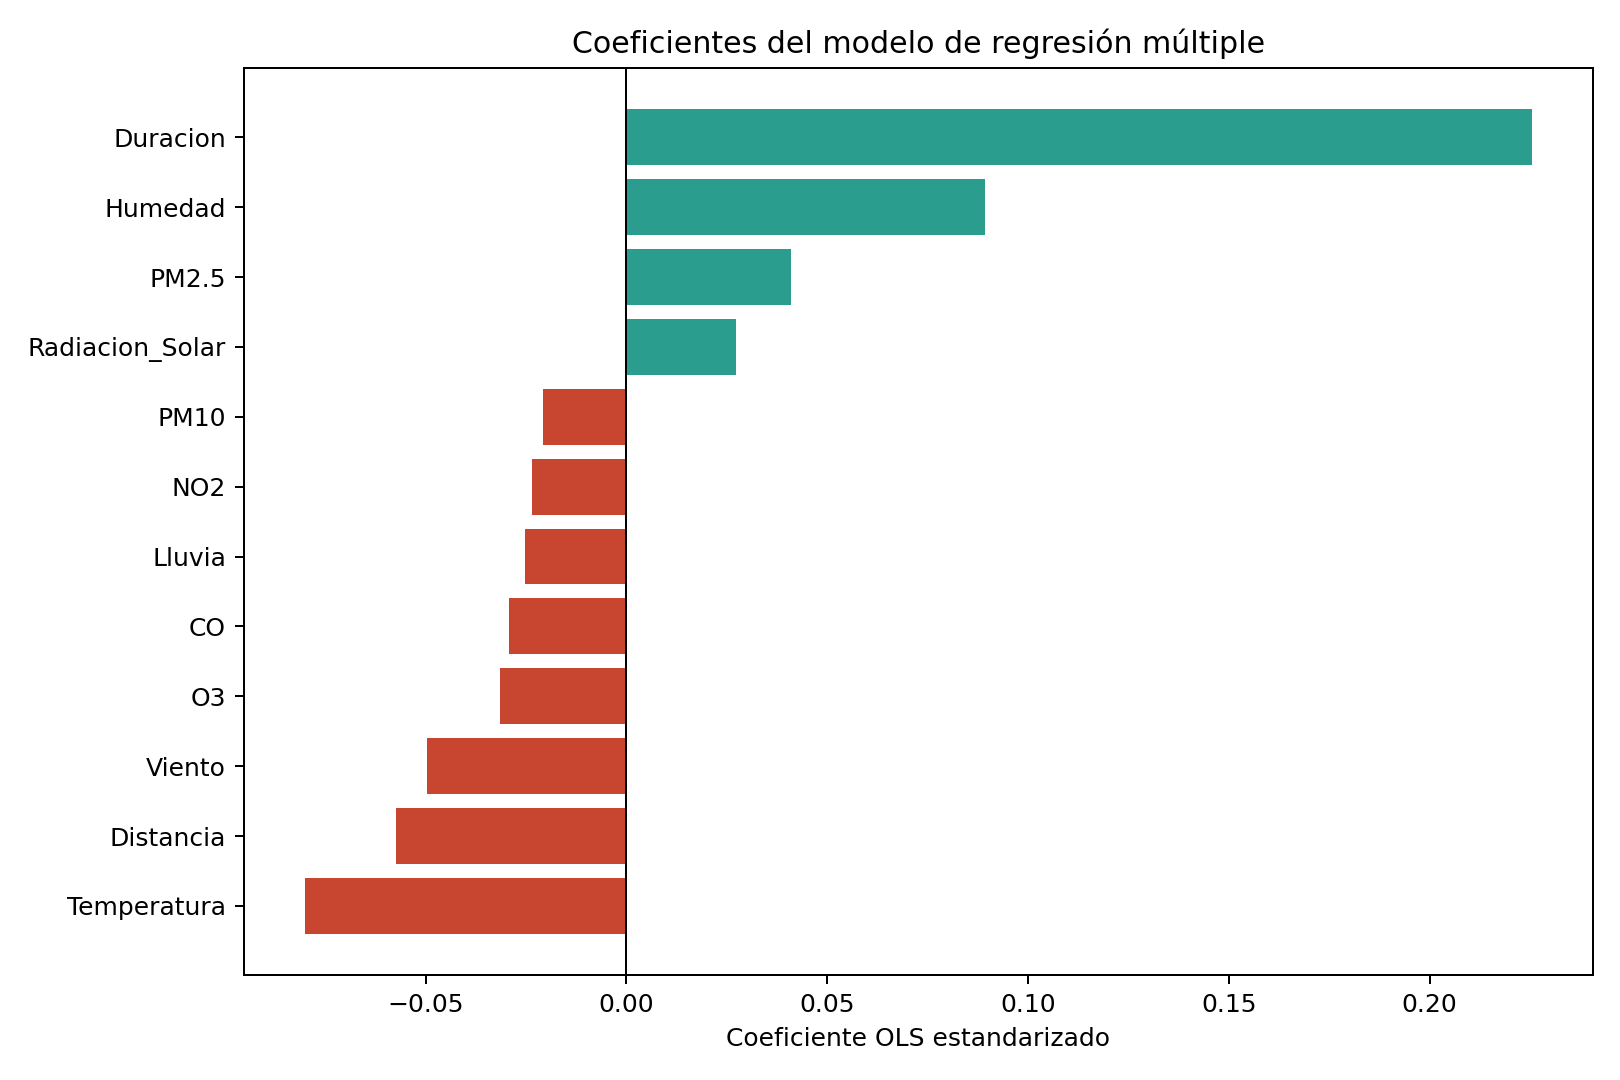
\includegraphics[width=\textwidth]{imagenes/regression_coefficients.png}
        \caption{Magnitud de coeficientes estandarizados del modelo de regresión.}
    \end{minipage}\hfill
    \begin{minipage}{0.48\textwidth}
        \centering
        
\includegraphics[width=\textwidth]{Informe/imagenes/02_regression_ci_coefficients.png}
        \caption{Coeficientes e intervalos de confianza HC3.}
    \end{minipage}

\end{figure}

\subsection{PCA, PPCA y análisis factorial}

La reducción de dimensión se hizo sobre nueve variables ambientales continuas estandarizadas. PCA retuvo tres componentes que explican el 80.63\% de la variabilidad: PC1=45.87\%, PC2=27.52\% y PC3=7.24\%. PC1 representó un gradiente climático-fotoquímico con humedad opuesta a temperatura, O3, viento y radiación. PC2 representó el material particulado, dominado por PM2.5 y PM10. PC3 capturó gases de combustión, con señal de NO2 y CO.

\begin{figure}[H]
\centering
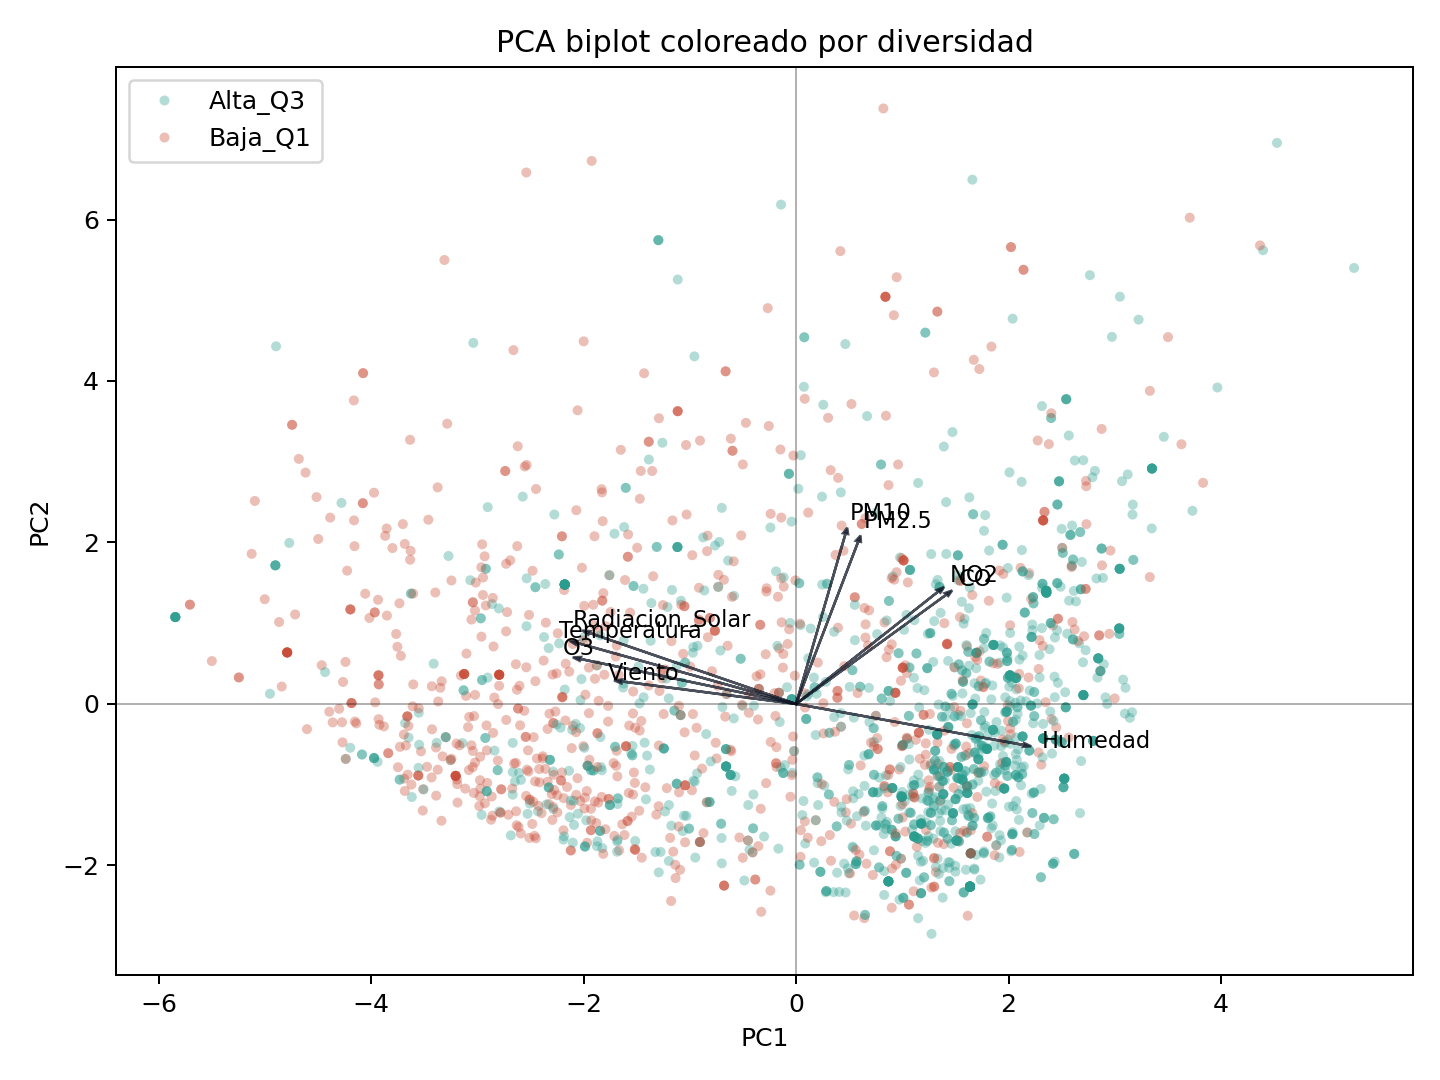
\includegraphics[width=0.48\linewidth]{imagenes/pca_biplot_q1_q3.png}

\includegraphics[width=0.48\linewidth]{Informe/imagenes/Cargas_PCA.png}
\caption{Izquierda: biplot PCA por extremos de diversidad. Derecha: cargas factoriales Varimax.}
\end{figure}

PPCA formuló la estructura como modelo generativo con tres causas latentes y ruido isotrópico ($\sigma^2=0.291$). En la matriz generativa $W$, la dimensión climática aumentó humedad y redujo temperatura, O3, radiación y viento; la dimensión de partículas elevó PM2.5 y PM10; y la de gases elevó NO2 y CO.

\begin{figure}[H]
\centering

\includegraphics[width=0.52\linewidth]{Informe/imagenes/Heatmap PPCA.png}
\caption{Cargas de cada variable latente sobre las variables originales mediante PPCA.}
\end{figure}

En análisis factorial con rotación Varimax los factores fueron más interpretables: Factor~1 material particulado (PM2.5=0.970, PM10=0.802); Factor~2 clima/fotoquímica (temperatura=0.926, humedad=$-$0.906, radiación=0.864, O3=0.788); Factor~3 gases locales (NO2=0.711, CO=0.647). PM2.5, temperatura y humedad presentaron alta comunalidad, mientras viento tuvo la menor ($0.354$), lo que indica que su varianza está poco capturada por los tres ejes comunes.

\begin{figure}[H]
\centering
\begin{minipage}[c]{0.52\linewidth}
\centering

\includegraphics[width=0.95\linewidth]{Informe/imagenes/fa_varimax_loadings.png}
\caption{Cargas Varimax sobre variables originales.}
\end{minipage}
\hfill
\begin{minipage}[c]{0.40\linewidth}
\centering
\scriptsize
\captionof{table}{Comunalidad y unicidad en el análisis factorial.}
\vspace{0.15cm}
\begin{tabular}{lrr}
\toprule
Variable & Comunalidad & Unicidad \\
\midrule
PM2.5 & 0.956 & 0.044 \\
PM10 & 0.730 & 0.270 \\
NO2 & 0.696 & 0.304 \\
CO & 0.648 & 0.352 \\
O3 & 0.700 & 0.300 \\
Temperatura & 0.860 & 0.140 \\
Humedad & 0.854 & 0.146 \\
Viento & 0.354 & 0.646 \\
Radiación solar & 0.753 & 0.247 \\
\bottomrule
\end{tabular}
\end{minipage}
\end{figure}

Los errores de reconstrucción complementan la interpretación metodológica: FA reconstruyó mejor la covarianza (Frobenius=0.141 vs. PPCA=0.385), mientras PCA obtuvo el menor MSE de datos (0.194), seguido de PPCA (0.214) y FA (0.220). PCA es más eficiente para compresión; FA representa mejor la estructura de covarianza común bajo factores interpretables; PPCA ofrece una lectura generativa intermedia.

\begin{table}[H]
\centering
\caption{Errores de reconstrucción de covarianza y de datos.}
\footnotesize
\begin{tabular}{lrr}
\toprule
Modelo & Error covarianza & MSE datos \\
\midrule
PCA (3 comp.) & -- & 0.194 \\
PPCA & 0.385 & 0.214 \\
Factor Analysis & 0.141 & 0.220 \\
\bottomrule
\end{tabular}
\end{table}

\section{Discusión}

\subsection{Inferencia permutacional: la firma ambiental de los microhábitats}

La prueba permutacional de distancia entre centroides (5\,000 simulaciones; distancia observada$=1.921$, $p<0.001$) demostró que los ambientes asociados a alta y baja diversidad de aves ocupan regiones distinguibles del espacio multivariado de nueve variables, incluso cuando los supuestos gaussianos del Hotelling $T^2$ clásico son violados. La separación es simultánea en temperatura, humedad, O3, viento y radiación solar, lo que indica que la diversidad responde a una \textit{firma ambiental integrada} y no a efectos de una sola variable.

Ecológicamente, esa firma corresponde a tipos reconocibles de microhábitat urbano. El perfil de alta diversidad ---frío, húmedo, con baja radiación y bajo ozono--- es propio de las primeras horas de la mañana en humedales, parques arbolados y laderas de los cerros orientales de Bogotá, donde la cobertura vegetal retiene humedad, amortigua la temperatura y provee refugio, alimento (artrópodos, frutos, néctar) y perchas diversas para aves residentes y migratorias. El perfil de baja diversidad ---caliente, seco, con alta insolación y O3 elevado--- es característico de superficies pavimentadas y corredores viales en las horas centrales del día, donde el efecto de isla de calor urbana es más intenso. La diferencia de 4 °C entre perfiles (12.9 vs. 16.8 °C) es ecológicamente significativa a 2\,600 m s.n.m., donde los rangos térmicos intradiurnos son amplios y las aves son sensibles a variaciones horarias. La distribución conjunta temperatura--humedad--Shannon refuerza este mecanismo: la esperanza condicional bajo la normal trivariada confirmó que Shannon esperado aumenta a medida que la temperatura cae y la humedad sube ($R^2\approx0.124$), capturando exclusivamente el componente climático de la diversidad.

\subsection{Regresión múltiple: esfuerzo, clima y contaminación como predictores independientes}

La regresión lineal múltiple ($R^2=0.289$, $n=5{,}298$, $F=179.4$, $p<0.001$) permitió separar la contribución del esfuerzo del observador de la señal ambiental real. La duración de la observación fue el predictor más fuerte ($\beta=0.225$), reflejando el efecto clásico de las curvas de acumulación de especies: listas más largas detectan especies raras, crípticas o de hábito silencioso de forma independiente al ambiente. Adicionalmente, los observadores más dedicados tienden a salir temprano ---cuando el ambiente es más frío y húmedo--- y a permanecer más tiempo, generando una correlación espuria entre esfuerzo y condiciones climáticas si no se controla explícitamente. El hallazgo crítico es que, incluso después de controlar por duración y distancia recorrida, humedad ($\beta=0.089$), temperatura ($\beta=-0.080$), viento ($\beta=-0.050$), O3 ($\beta=-0.032$), CO ($\beta=-0.029$), lluvia ($\beta=-0.025$) y NO2 ($\beta=-0.023$) mantuvieron efectos significativos con errores robustos HC3: la señal ambiental es real.

La humedad actúa como proxy de integridad vegetal: mayor cobertura arbórea implica más retención de humedad, mayor abundancia de artrópodos y más nichos de anidación; su fuerte covarianza negativa con temperatura (cov$=-55.221$) hace que ambas variables actúen sinérgicamente, amplificando el gradiente de diversidad. El O3 es un contaminante secundario formado por fotólisis del NO2 bajo alta radiación UV al mediodía; su colinealidad con temperatura y radiación (todos en PC1/Factor~2 Varimax) implica que su coeficiente de regresión subestima su efecto ecológico total, del que parte queda capturado por las otras dos variables. A nivel fisiológico, el O3 es tóxico para el aparato respiratorio de las aves y daña la vegetación que sostiene a las aves insectívoras. NO2 y CO son trazadores de corredores viales de alta densidad de tráfico, entornos con escasa cobertura vegetal donde el ruido y el movimiento vehicular inhiben la actividad avifaunística. El signo positivo de PM2.5 ($\beta=0.041$) es contraintuitivo pero coherente con el crecimiento higroscópico de las partículas finas en condiciones de alta humedad, precisamente el ambiente asociado a mayor diversidad; el coeficiente refleja así una confusión parcial con la humedad más que un efecto biológico directo. Finalmente, la distancia a la estación RMCAB ($\beta=-0.057$) indica un sesgo espacial: las estaciones están ubicadas en sectores urbanos densos y degradados, de modo que las listas eBird en su entorno inmediato corresponden a microhábitats menos diversos que los alejados de ellas.

\subsection{Reducción de dimensión: estructura latente y tipos de microhábitat urbano}

PCA, PPCA y FA convergieron en identificar tres dimensiones latentes que explican el 80.63\% de la variabilidad de las nueve variables ambientales. El eje climático-fotoquímico (PC1=45.87\%; Factor~2 Varimax: temperatura=0.926, humedad=$-$0.906, radiación=0.864, O3=0.788) es el dominante y opone microhábitats vegetados ---frescos, húmedos, con baja radiación--- a superficies impermeables y abiertas. El eje de material particulado (PC2=27.52\%; Factor~1 Varimax: PM2.5=0.970, PM10=0.802) refleja la proximidad a vías de alta circulación, industria y construcción. El eje de gases de combustión (PC3=7.24\%; Factor~3 Varimax: NO2=0.711, CO=0.647) captura la intensidad local del tráfico, independientemente de la carga de partículas. El biplot confirmó que los registros de alta diversidad se agrupan en el cuadrante húmedo-fresco-bajo O3, sin solapamiento sustancial con el cuadrante opuesto donde se concentran los de baja diversidad. La baja comunalidad del viento (0.354) indica que su variabilidad está determinada por factores topográficos locales no compartidos con los demás predictores, lo que explica también por qué su efecto individual en regresión es más variable entre especificaciones. En términos de rendimiento, FA minimizó el error de reconstrucción de covarianza (Frobenius=0.141 vs. PPCA=0.385), siendo el más adecuado para interpretar la estructura común; PCA minimizó el MSE de datos (0.194), siendo el más eficiente para compresión; y PPCA cuantificó explícitamente la variabilidad no explicada por los factores latentes mediante su ruido isotrópico ($\sigma^2=0.291$).

\section{Conclusiones}

El análisis multivariado confirmó que la diversidad de aves en Bogotá responde a una firma ambiental integrada: los microhábitats frescos, húmedos y con baja radiación y ozono ---humedales, parques arbolados y laderas en horas tempranas--- concentran la mayor riqueza avifaunística, mientras los entornos cálidos, secos y fotoquímicamente activos del mediodía urbano corresponden a la menor diversidad. Esta separación es estadísticamente robusta (prueba permutacional, $p<0.001$) y persiste tras controlar por esfuerzo de muestreo en la regresión múltiple, descartando que los patrones sean artefactos de la ciencia ciudadana. El esfuerzo de observación (duración, $\beta=0.225$) es el predictor más fuerte, pero humedad, temperatura, O3, viento, CO, NO2 y lluvia retienen efectos significativos con errores robustos HC3, lo que confirma que la señal ambiental es real. La reducción de dimensión reveló tres ejes interpretables ---clima/fotoquímica, partículas y gases de combustión--- que explican el 80\% de la variabilidad ambiental y se corresponden con tipos reales de microhábitat bogotano.

\end{document}
